\subsection{2026-09-21 --- Does more capacity fix the multi-output model's regressed units?}
\label{sec:capacity}

\subsubsection*{Goal.} Section~\ref{sec:multioutput} flagged, but did not test, the hypothesis
that Songa\_G1 and Lio\_G1 regressed under the joint multi-output model because 200 trees
shared across 14 outputs gives far less dedicated capacity per unit than baseline 1's
200-trees-\emph{each}. Full notebook: \texttt{src/modeling/multioutput\_tree\_capacity.ipynb}.

\subsubsection*{Method.} Trained once to 3{,}000 trees (no early stopping; see below for why),
identical features/hyperparameters to Section~\ref{sec:multioutput} otherwise. Checked the
official \texttt{kaggle\_metric.py} micro-AUC at $\sim$45 checkpoints via
\texttt{predict\_proba(..., iteration\_range=(0,k))}, which reuses the one trained model rather
than retraining at every candidate tree count.

\finding{XGBoost's own multi-output \texttt{eval\_metric="auc"} does \emph{not} match the
official micro-AUC --- it tracks consistently lower and noisier (Figure~\ref{fig:capacity-internal}).
Almost certainly a macro-average across the 14 outputs rather than a pooled/micro calculation.
Using it for early stopping in this multi-output setup would optimize the wrong target, which is
why this run used a fixed generous cap and our own checkpointing instead.}

\begin{figure}[htbp]
  \centering
  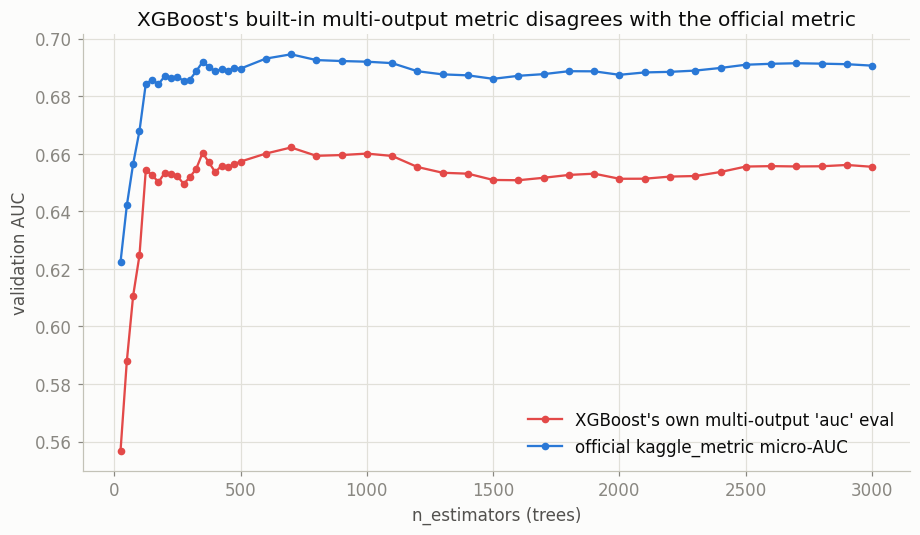
\includegraphics[width=0.8\linewidth]{figures/capacity_01_internal_vs_official.png}
  \caption{XGBoost's internal multi-output AUC vs.\ the official micro-AUC.}
  \label{fig:capacity-internal}
\end{figure}

\subsubsection*{Results: a real plateau, then a real decline.}

\begin{figure}[htbp]
  \centering
  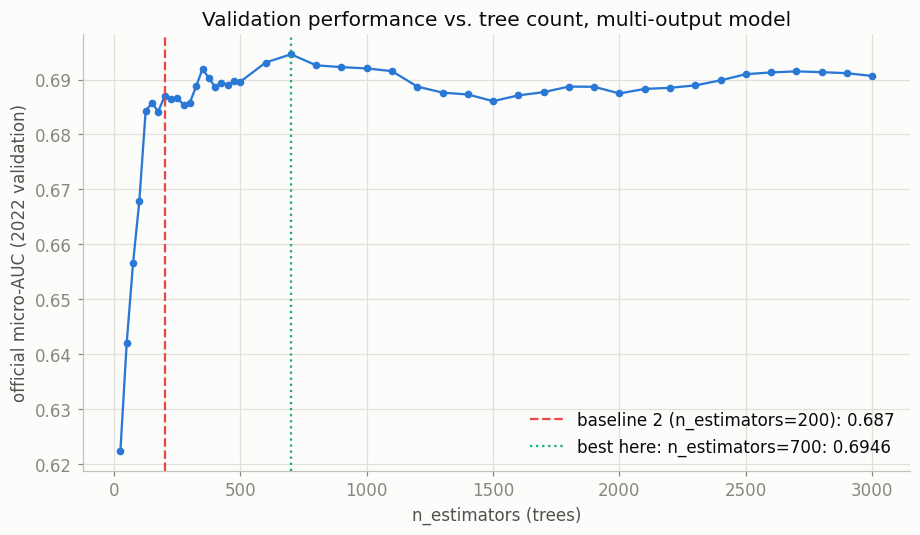
\includegraphics[width=0.8\linewidth]{figures/capacity_02_plateau_curve.png}
  \caption{Official micro-AUC vs.\ tree count, up to 3{,}000 trees.}
  \label{fig:capacity-plateau}
\end{figure}

\finding{Validation performance rises sharply to $\sim$150 trees, keeps climbing gently to a
peak at \textbf{$n_{\text{estimators}}=700$ (micro-AUC 0.6946)}, then genuinely declines to
$\sim$0.686 by 1{,}500 trees --- a real $\sim$0.008 drop, not noise --- before a mild, incomplete
recovery out to 3{,}000 that never regains the 700-tree peak (Figure~\ref{fig:capacity-plateau}).
$n_{\text{estimators}}=700$ is a $+0.0076$ improvement over baseline 2's original
$n_{\text{estimators}}=200$ (0.687 $\to$ 0.6946), confirming the model was undertrained, not
just differently structured.}

\begin{figure}[htbp]
  \centering
  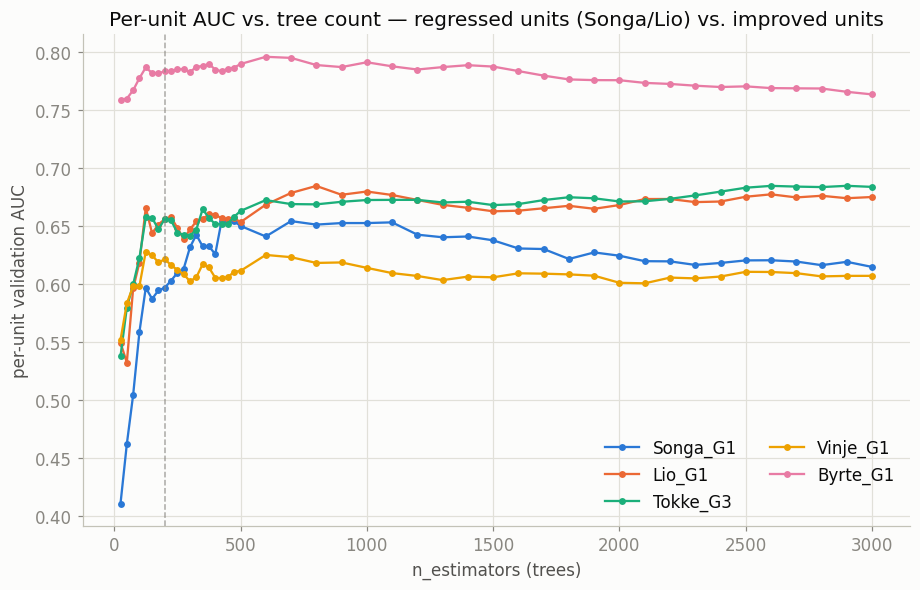
\includegraphics[width=0.8\linewidth]{figures/capacity_03_per_unit_curves.png}
  \caption{Per-unit AUC vs.\ tree count: regressed units (Songa\_G1, Lio\_G1) vs.\ improved/strong units.}
  \label{fig:capacity-per-unit}
\end{figure}

\finding{\textbf{The capacity hypothesis is only partially right.} At $n_{\text{estimators}}=700$,
Songa\_G1 recovers from 0.597 (at 200 trees) to 0.655, and Lio\_G1 from 0.656 to 0.679
(Figure~\ref{fig:capacity-per-unit}) --- real improvement. But neither returns to its baseline-1
independent-model score (Songa\_G1: 0.677, Lio\_G1: 0.713) anywhere in the swept range; both
plateau and then decline alongside the overall curve rather than continuing to close the gap.
So: more capacity was genuinely part of the story, but something else about joint modeling still
costs these two specific units relative to modeling them independently. Left as an open question
for the next round of exploratory analysis rather than chased further here.}

\subsubsection*{Decision: adopt $n_{\text{estimators}}=300$, not the argmax.}
The sweep's argmax is 700, but the whole region from $\sim$125 to $\sim$500 trees is a noisy
plateau spanning only $\sim$0.006 AUC, measured on a \emph{single} validation year. Selecting the
argmax of a noisy validation curve is itself a form of overfitting --- to the validation set
rather than the training set --- and 700 would likely not be the argmax on a different holdout
year. We therefore adopt \textbf{$n_{\text{estimators}}=300$} as the standing default: inside the
stable plateau, cheaper to train, and not tuned to a single noisy peak. Measured score at 300 is
0.6858, nominally $0.0012$ below the $n=200$ run --- a difference well inside the noise of this
plateau, and not treated as meaningful. Revisit once there is a more robust validation scheme
(multiple holdout years or proper time-series CV) that could distinguish these points.

Updated in \texttt{report/leaderboard.md} as \texttt{xgb\_multioutput\_tree\_n700}.
